\section[Damped forms and sharp coercivity]{Basepoints: damped forms, multipliers and sharp coercivity}\label{yo:sec:damped}

The Thorin programme of this book leaves the critical line for a basepoint $\alpha>\frac12$, where the Thorin density of the shifted clock is $\rho_{\alpha-1/2}=\pi^{-1}\re\frac{\xi'}\xi(\alpha+i\tau)$ (equation~\eqref{eq:rho}). On Yoshida's side the same move damps the autocorrelation $\varphi*\widetilde\varphi$ by $e^{-(\alpha-1/2)|y|}$.

\subsection{The multiplier identity}\label{yo:sec:mult}

For a basepoint $\alpha\ge\frac12$ put $\varepsilon=\alpha-\frac12$ and define the damped Yoshida form
\[
\langle\varphi_1,\varphi_2\rangle_\alpha=\mathcal Y\bigl(e^{-\varepsilon|y|}\,\varphi_1*\widetilde{\varphi_2}\bigr),
\]
where $\mathcal Y$ is the functional of \eqref{yo:EF} and $\widetilde\varphi(y)=\overline{\varphi(-y)}$; at $\alpha=\frac12$ it is the form of Section~\ref{yo:sec:yoshida}, and $C(a)\subset K(a)$ are the spaces of that section. On the prime side the damping replaces $\Lambda(n)n^{-1/2}$ by $\Lambda(n)n^{-\alpha}$, and in the pole term $e^{y/2}+e^{-y/2}$ becomes $e^{(1-\alpha)|y|}+e^{-\alpha|y|}$; on $K(a)$ the prime sum is still finite, since only $\log n\le2a$ occurs. Let $\sigma_{\max}=\sup_\rho\re\rho\in[\frac12,1]$, let $v_\alpha(\tau)=\re\frac{\xi'}\xi(\alpha+i\tau)$ and $b_\alpha=v_\alpha(0)=\xi'(\alpha)/\xi(\alpha)$, so that $\rho_\varepsilon=\pi^{-1}v_{1/2+\varepsilon}$ is the density \eqref{eq:rho}, and write $P_w(\tau)=w/(\pi(w^2+\tau^2))$ for the Poisson kernel of width $w$, with $P_{-w}=-P_w$, as in Proposition~\ref{prop:struct}.

\begin{proposition}\label{yo:prop:mult}
Let $\alpha\ge\sigma_{\max}$, and suppose that no zero has real part $\alpha$. Then $\rho_\varepsilon$ is real analytic and positive, $(1+\tau^2)^{-1}\rho_\varepsilon$ is integrable over $\R$, and for every $a>0$ and every $\varphi\in K(a)$
\[
\langle\varphi,\varphi\rangle_\alpha=\int_{\R}|\widehat\varphi(\tau)|^2\,\rho_\varepsilon(\tau)\,d\tau=\frac1\pi\int_{\R}|\widehat\varphi(\tau)|^2\,v_\alpha(\tau)\,d\tau .
\]
\end{proposition}

\begin{proof}
For $w>0$ the kernel $P_w$ has Fourier transform $\int P_w(\tau)e^{i\tau y}\,d\tau=e^{-w|y|}$, so for a bounded $F$ with compact support and $\gamma\in\R$, $\int\widehat F(\tau)P_w(\tau-\gamma)\,d\tau=\int F(y)e^{-w|y|}e^{i\gamma y}\,dy$. Let $F=\varphi*\widetilde\varphi$, which is continuous, piecewise smooth and supported in $[-2a,2a]$, so that \eqref{yo:EF} applies to $e^{-\varepsilon|y|}F$ and
\[
\mathcal Y(e^{-\varepsilon|y|}F)=\sum_\rho\int F(y)e^{-\varepsilon|y|}e^{i\gamma_\rho y}\,dy,
\]
the series converging absolutely. Group the zeros in fours $\{\rho,\bar\rho,1-\rho,1-\bar\rho\}$, counted with multiplicity; for a zero on the critical line the group is $\{\rho,\bar\rho\}$. For the four zeros $\frac12\pm\delta\pm i\gamma$ with $\gamma>0$ and $\delta>0$ we have $e^{i\gamma_\rho y}=e^{\pm i\gamma y}e^{\pm\delta y}$, so their contributions add up to
\[
\begin{split}
&\int F(y)e^{-\varepsilon|y|}\bigl(e^{i\gamma y}+e^{-i\gamma y}\bigr)\bigl(e^{\delta y}+e^{-\delta y}\bigr)dy\\
&\quad=\int F(y)\bigl(e^{-(\varepsilon-\delta)|y|}+e^{-(\varepsilon+\delta)|y|}\bigr)\bigl(e^{i\gamma y}+e^{-i\gamma y}\bigr)dy,
\end{split}
\]
because $e^{\delta y}+e^{-\delta y}$ is even. The widths $\varepsilon-\delta=\alpha-\beta$ and $\varepsilon+\delta=\alpha-(1-\beta)$, with $\beta=\frac12+\delta$, are the differences between $\alpha$ and the real parts of the zeros of the group, and they are positive, since every zero has real part less than $\alpha$. By the identity for $P_w$ the group contributes $\int\widehat F(\tau)\sum P_{\alpha-\beta_{\rho'}}(\tau-\im\rho')\,d\tau$, the sum over its four members $\rho'$ with real part $\beta_{\rho'}$; the same holds for a zero on the line, with the single width $\varepsilon$. Hence $\mathcal Y(e^{-\varepsilon|y|}F)=\sum_\rho\int\widehat F(\tau)P_{\alpha-\beta_\rho}(\tau-\im\rho)\,d\tau$ over all zeros, where $\beta_\rho=\re\rho$. Now $\widehat F=|\widehat\varphi|^2\ge0$ on $\R$, so every term is nonnegative and the sum and the integral may be interchanged. By Proposition~\ref{prop:struct}, which is Hadamard's product, $\sum_\rho P_{\alpha-\beta_\rho}(\tau-\im\rho)=\pi^{-1}\re\frac{\xi'}\xi(\alpha+i\tau)=\rho_\varepsilon(\tau)$, a sum of positive kernels; it is real analytic because no zero lies on the line $\re s=\alpha$. Finally $\int P_w(\tau-t)(1+\tau^2)^{-1}d\tau=(1+w)/((1+w)^2+t^2)\le(1+\alpha)/(1+t^2)$ for $0<w\le\alpha$, so by Tonelli $\int(1+\tau^2)^{-1}\rho_\varepsilon\,d\tau\le(1+\alpha)\sum_\rho(1+(\im\rho)^2)^{-1}<\infty$, because the number of zeros with $|\im\rho|\le T$ is $O(T\log T)$. The proof used only that $F=\varphi*\widetilde\varphi$ is continuous, piecewise $C^1$ and supported in $[-2a,2a]$, so the identity holds as well for every bounded piecewise $C^1$ function $\varphi$ supported in $[-a,a]$.
\end{proof}

For the Fej\'er taper $\varphi=e^{ity}\chi_0$ on the window $a=X/2$ one has $\varphi*\widetilde\varphi=e^{ity}(1-|y|/X)_+$, and since $\mathcal Y(F)$ depends only on the even part of $F$, $\langle\varphi,\varphi\rangle_\alpha=\mathcal Y\bigl(e^{-\varepsilon|y|}\cos(ty)(1-|y|/X)_+\bigr)=2A_X(\varepsilon,t)$ in the notation of Proposition~\ref{mw:prop:AX}, whose part (c), $A_X(\varepsilon,t)\to v_\alpha(t)$ as $X\to\infty$ when $\alpha>\sigma_{\max}$, so that every zero has $|\beta-\frac12|<\varepsilon$, is the concentration argument in the proof of Theorem~\ref{yo:thm:coercive}(i) below for this family of test functions.

\begin{remark}\label{yo:rem:mult}
For $\alpha<\sigma_{\max}$ the two sides of the identity differ: a zero with $\beta>\alpha$ contributes the growing factor $e^{(\beta-\alpha)|y|}$ to the damped Weil form, but the negative kernel $P_{\alpha-\beta}=-P_{\beta-\alpha}$ to the symbol. The script \texttt{yo\_damped.py} checks the identity at $\alpha=1$, $a=0.8$ and $\varphi=\chi_0$ (data in \texttt{yo\_damped.json}, \texttt{code/\allowbreak README.md}).
\end{remark}

\begin{theorem}\label{yo:thm:damped}
The damped forms have the following properties.
\begin{enumerate}
\item[(i)] For $\alpha\ge\sigma_{\max}$ the damped form is positive semidefinite on $C_c^\infty(\R)$; unconditionally this holds for every $\alpha\ge1$.
\item[(ii)] RH holds if and only if the damped form is positive semidefinite for every $\alpha>\frac12$.
\item[(iii)] If the damped form at $\alpha$ is positive semidefinite on $C(a)$, so is the form at every $\alpha'>\alpha$; thus $a_0(\alpha)=\sup\{a:\langle\cdot,\cdot\rangle_\alpha\ge0\text{ on }C(a)\}$ is nondecreasing in $\alpha$.
\end{enumerate}
\end{theorem}

\begin{proof}
(i) If no zero has real part $\alpha$ this is Proposition~\ref{yo:prop:mult}, because $\rho_\varepsilon\ge0$ and every $\varphi\in C_c^\infty(\R)$ lies in some $K(a)$. If a zero has real part $\alpha$, then $\alpha=\sigma_{\max}$ and $\langle\varphi,\varphi\rangle_\alpha=\lim_{\alpha'\downarrow\alpha}\langle\varphi,\varphi\rangle_{\alpha'}\ge0$, since for fixed $\varphi$ each part of the form is continuous in $\varepsilon$: the pole term and the finite prime sum obviously, and $V_1(e^{-\varepsilon|y|}F)$ because $\widehat{e^{-\varepsilon|y|}F}=P_\varepsilon*\widehat F$ with $|\widehat F(t)|\le C(1+t^2)^{-1}$, which gives a bound $C'(1+t^2)^{-1}$ uniform in $\varepsilon\le1$, while $\re\psi(\frac14+\frac{it}2)=O(\log(2+|t|))$, and dominated convergence applies to the Fourier form of $V_1$ in \eqref{yo:V1}. Unconditionally $\sigma_{\max}\le1$ and no zero has real part $1$, so every $\alpha\ge1$ is covered.

(ii) Under RH, $\sigma_{\max}=\frac12$ and (i) applies to every $\alpha>\frac12$. Conversely, positivity for a sequence $\alpha_n\downarrow\frac12$ gives $\langle\varphi,\varphi\rangle\ge0$ for every $\varphi\in C_c^\infty(\R)$ by the same continuity, which is Weil's criterion (Section~\ref{yo:sec:yoshida}).

(iii) Write $e^{-\varepsilon'|y|}=\int P_{\varepsilon'}(\lambda)e^{i\lambda y}\,d\lambda$ with $\varepsilon'=\alpha'-\alpha$. Since $(\varphi_\lambda*\widetilde{\varphi_\lambda})(y)=e^{i\lambda y}(\varphi*\widetilde\varphi)(y)$ for $\varphi_\lambda=e^{i\lambda y}\varphi\in C(a)$, we get $\langle\varphi,\varphi\rangle_{\alpha'}=\int P_{\varepsilon'}(\lambda)\langle\varphi_\lambda,\varphi_\lambda\rangle_\alpha\,d\lambda$ (Fubini, as in (i)), which is nonnegative when the form at $\alpha$ is positive semidefinite on $C(a)$.
\end{proof}

\begin{remark}[One basepoint]\label{yo:rem:single}
Part (ii) uses every $\alpha>\frac12$. The converse of (i) holds at a single basepoint: if $\frac12\le\alpha\le1$ and $\langle\varphi,\varphi\rangle_\alpha\ge0$ for every $\varphi\in C_c^\infty(\R)$, then no zero has real part greater than $\alpha$. This is Theorem~\ref{dc:thm:damped} of Chapter~\ref{chap:dc}. With (i), the damped form at $\alpha\in[\frac12,1]$ is positive semidefinite if and only if $\sigma_{\max}\le\alpha$. A statement about the symbol on one line is weaker: positivity of $v_\alpha$ on the line $\re s=\alpha$ is not known to exclude zeros to its right (Remark~\ref{rem:ch2:oneline}).
\end{remark}

\subsection{Sharp coercivity}\label{yo:sec:coercive}

For $a>0$ let
\[
\lambda_{\min}(\alpha,a)=\inf\Bigl\{\frac{\langle\varphi,\varphi\rangle_\alpha}{\|\varphi\|^2}:\ 0\ne\varphi\in K(a)\Bigr\},
\]
the least eigenvalue of the damped form on the window $[-a,a]$, where $\|\cdot\|$ is the norm of $L^2(\R)$ and the test functions are complex valued. The matrix of the form on the basis $\chi_n$, $|n|\le N$, is the form restricted to a subspace of $K(a)$, so its least eigenvalue is an upper bound for $\lambda_{\min}(\alpha,a)$: these are the finite sections of Table~\ref{yo:tab:lam}. Under the hypotheses of Proposition~\ref{yo:prop:mult} the infimum over the smaller space $C(a)$ is the same. Indeed, let $\varphi\in K(a)$ and let $\psi_\delta\in C_c^\infty(-a,a)$ satisfy $0\le\psi_\delta\le1$ and $\psi_\delta=1$ on $[-a+\delta,a-\delta]$, with $\psi_\delta$ monotone on each of the two end intervals. Then $\eta_\delta=\varphi(1-\psi_\delta)$ lies in $K(a)$, has total variation bounded independently of $\delta$ and $L^1$ norm at most $2\delta\|\varphi\|_\infty$, so that $|\widehat{\eta_\delta}(\tau)|\le C\min(\delta,|\tau|^{-1})$, and $\langle\eta_\delta,\eta_\delta\rangle_\alpha=\int|\widehat{\eta_\delta}|^2\rho_\varepsilon\to0$ as $\delta\downarrow0$ by dominated convergence, since $(1+\tau^2)^{-1}\rho_\varepsilon$ is integrable. The form being positive semidefinite on $K(a)$, the Rayleigh quotients of $\varphi\psi_\delta\in C(a)$ tend to that of $\varphi$. The argument applies verbatim to the functions supported in $[-a,a]$ that are smooth on $[-a,a]$, to which Proposition~\ref{yo:prop:mult} extends, so the infimum is the same over that larger class; it contains the Legendre polynomials on the window used in Chapter~\ref{chap:dc}, whose finite sections are therefore upper bounds as well. Put $m_\alpha=\inf_{\tau\in\R}v_\alpha(\tau)$.

\begin{theorem}\label{yo:thm:coercive}
Let $V_\xi=(\log\xi)''(\frac12)$ and $p_1=\frac12V_\xi=0.0231049931\ldots$, which is $\sum_{\gamma>0}\gamma^{-2}$ under RH, and, under RH, let $p_2=\sum_{\gamma>0}\gamma^{-4}=3.71726\ldots\times10^{-5}$.
\begin{enumerate}
\item[(i)] If $\alpha\ge\sigma_{\max}$ and no zero has real part $\alpha$, then $\lambda_{\min}(\alpha,a)\ge2m_\alpha$ for every $a>0$, $\lambda_{\min}(\alpha,a)$ is nonincreasing in $a$, and $\lambda_{\min}(\alpha,a)\to2m_\alpha$ as $a\to\infty$.
\item[(ii)] Under RH, $m_\alpha=b_\alpha=\xi'(\alpha)/\xi(\alpha)$ for every $\alpha>\frac12$, and $v_\alpha(\tau)>b_\alpha$ for $\tau\ne0$: the minimum of $\re\xi'/\xi$ on each vertical line lies on the real axis, and only there. For $\alpha\ge1$ this holds with no hypothesis (Proposition~\ref{bp:prop:valpha}, and Proposition~\ref{bp:prop:v1min} for $\alpha=1$); for $\frac12<\alpha<1$ it holds with no hypothesis for $0<|\tau|\le3\times10^{12}-1.21$ (Theorem~\ref{thm:dbeta:minall}(ii)); and RH is equivalent to it on every line $\frac12<\alpha<1$ (Theorem~\ref{thm:dbeta:minall}(vi), which sharpens Lagarias's criterion \cite{Lagarias}).
\item[(iii)] Hence RH holds if and only if
\[
\langle\varphi,\varphi\rangle_\alpha\ \ge\ 2b_\alpha\,\|\varphi\|^2\qquad\text{for all }\alpha\in(\tfrac12,1],\ a>0,\ \varphi\in K(a),
\]
and under RH the constant is sharp: $\lambda_{\min}(\alpha,a)\downarrow2b_\alpha$ as $a\to\infty$.
\item[(iv)] For every $\alpha>\frac12$, with no hypothesis, $2b_\alpha\le4p_1(\alpha-\frac12)$; under RH also $4p_1(\alpha-\frac12)-4p_2(\alpha-\frac12)^3\le2b_\alpha$. The coercivity constant vanishes linearly at $\alpha=\frac12$.
\end{enumerate}
\end{theorem}

\begin{proof}
(i) By Proposition~\ref{yo:prop:mult} and Plancherel, $\int|\widehat\varphi|^2=2\pi\|\varphi\|^2$, we have, for $\varphi\in K(a)$,
\[
\langle\varphi,\varphi\rangle_\alpha=\pi^{-1}\int|\widehat\varphi|^2v_\alpha\ge\pi^{-1}m_\alpha\int|\widehat\varphi|^2=2m_\alpha\|\varphi\|^2 .
\]
Monotonicity holds because $\lambda_{\min}(\alpha,a)$ is also the infimum over $C(a)$ and $C(a)\subset C(a')$ for $a<a'$. For the limit, fix $\tau_0$ and $\psi\in C_c^\infty(-1,1)$ with $\|\psi\|=1$, and let $\varphi_a(y)=a^{-1/2}e^{-i\tau_0y}\psi(y/a)\in C(a)$. Then $\|\varphi_a\|=1$, $|\widehat{\varphi_a}(\tau)|^2=a\,|\widehat\psi(a(\tau-\tau_0))|^2$, and $|\widehat{\varphi_a}|^2/2\pi$ is a probability density that concentrates at $\tau_0$ as $a\to\infty$. The function $v_\alpha$ is continuous and $(1+\tau^2)^{-1}v_\alpha$ is integrable (Proposition~\ref{yo:prop:mult}), and $\widehat\psi$ is a Schwartz function, so $\langle\varphi_a,\varphi_a\rangle_\alpha=\pi^{-1}\int|\widehat{\varphi_a}|^2v_\alpha\to2v_\alpha(\tau_0)$. Hence $\limsup_a\lambda_{\min}(\alpha,a)\le2v_\alpha(\tau_0)$ for every $\tau_0$, that is, $\le2m_\alpha$.

(ii) Under RH the whole of (ii) is in the book, at the places cited; for $\alpha\ge1$ no hypothesis is needed.

(iii) Under RH, (i) and (ii) give the inequality and its sharpness. Conversely, $b_\alpha>0$ for every $\alpha>\frac12$ with no hypothesis (Theorem~\ref{thm:dbeta:minall}(i)), so the inequality gives positive semidefiniteness for $\alpha\in(\frac12,1]$, Theorem~\ref{yo:thm:damped}(i) covers $\alpha>1$, and part (ii) of that theorem gives RH.

(iv) The upper bound is Theorem~\ref{thm:dbeta:minall}(i), $b_\alpha\le(\alpha-\frac12)V_\xi$, with $V_\xi=2p_1$. Under RH, $b_\alpha=\sum_{\gamma>0}2\varepsilon/(\varepsilon^2+\gamma^2)$ and $\gamma^{-2}-\varepsilon^2\gamma^{-4}\le(\varepsilon^2+\gamma^2)^{-1}\le\gamma^{-2}$.
\end{proof}

\begin{remark}\label{yo:rem:line}
At a single $\alpha\in(\frac12,1)$ with no zero on the line, the inequality $\langle\varphi,\varphi\rangle_\alpha\ge2b_\alpha\|\varphi\|^2$ for all $a$ and $\varphi$ holds if and only if $\sigma_{\max}\le\alpha$ and $v_\alpha\ge b_\alpha$ on the line: if it holds, the form is positive semidefinite (as $b_\alpha>0$), so $\sigma_{\max}\le\alpha$ by Remark~\ref{yo:rem:single}, and then (i) gives $2m_\alpha\ge2b_\alpha$, while $m_\alpha\le v_\alpha(0)=b_\alpha$; the converse is (i).
\end{remark}

\begin{lemma}\label{yo:lem:gap}
Consecutive ordinates of the zeros of $\zeta$ differ by at most $6.8874$. Hence every real $\tau$ with $|\tau|\ge\gamma_1$ lies within $3.4437$ of an ordinate.
\end{lemma}

\begin{proof}
The lemma needs no hypothesis on the zeros. The first $1800$ zeros of Proposition~\ref{bp:prop:v1min}, computed in ball arithmetic, reach height $2304.3$: consecutive ordinates among them differ by at most $\gamma_2-\gamma_1=6.88731\ldots$, and the later gaps by at most $5.4141$ (between $\gamma_3=25.0109$ and $\gamma_4=30.4249$). It remains to show that $\gamma'-\gamma\le h:=6.8874$ for consecutive ordinates $\gamma<\gamma'$ with $\gamma\ge2304.3$. Take $T$ with $\gamma<T<\gamma'$ and write $N(T)=\vartheta(T)/\pi+1+S(T)$ (Section~\ref{sec:ch5:turing}). The second derivative $\vartheta''(T)=\frac T4\sum_{k\ge0}(k+\frac14)\bigl((k+\frac14)^2+\frac{T^2}4\bigr)^{-2}$ is positive, so $\vartheta$ is convex, $\vartheta(T+h)-\vartheta(T)\ge h\vartheta'(T)$, and
\[
N(T+h)-N(T)\ \ge\ \frac{h\,\vartheta'(T)}\pi-|S(T)|-|S(T+h)| .
\]
We use the bounds of \cite{HSW22} as they are quoted in the proof of Proposition~\ref{bp:prop:v1min}: $|S(t)|\le2.5167$ for $0\le t\le X_0=30\,610\,046\,000$, and $|S(t)|\le B(t)=0.1095\log t+0.2042\log\log t+3.0305$ for $t\ge e$, with $B$ increasing. For $2304.3\le T\le X_0-h$ the first bound applies to both terms, and $\vartheta'(T)\ge\vartheta'(2304.3)=2.9523$ gives $N(T+h)-N(T)\ge6.4725-5.0334>1.4$. For $T>X_0-h$ both $|S(T)|$ and $|S(T+h)|$ are at most $B(T+h)$, because $B(X_0)=6.32>2.5167$, so $N(T+h)-N(T)\ge D(T)=h\vartheta'(T)/\pi-2B(T+h)$. At $T=X_0-h$, $h\vartheta'(T)/\pi=24.452$ and $2B(X_0)=12.649$, so $D(X_0-h)=11.80>0$; and $D$ increases, because a comparison of the sum for $\vartheta''$ with an integral gives $\vartheta''(T)\ge\frac1{2T}-\frac1{T^2}$, while $2T\,B'(T+h)\le0.219+0.4084/\log T$, so that $T\,D'(T)\ge\frac h{2\pi}(1-\frac2T)-0.219-\frac{0.4084}{\log T}>0.8$ for $T\ge X_0-h$. In every case $N(T+h)-N(T)>0$, so some ordinate lies in $(T,T+h]$, and letting $T\downarrow\gamma$ gives $\gamma'-\gamma\le h$. Finally, a real $\tau$ with $|\tau|\ge\gamma_1$ lies between two consecutive ordinates, hence within half a gap of one of them.
\end{proof}
% CHECK: the constants 2.5167, X_0 = 30 610 046 000, 0.1095, 0.2042 and 3.0305 of HSW22 are quoted from the proof of Proposition bp:prop:v1min (ch/basepoint.tex) and have not been rechecked against the paper by this editor; code/yo_gaps.py (checks-Y3.md) checks the arithmetic of this proof: threshold 619.994 for h = 6.8874, smallest step 5.356075 for T >= 2304.3, D(X_0 - h) = 11.8028, and a ball arithmetic grid above X_0 as a sanity check of D_h > 0 and D_h' > 0.

\begin{corollary}\label{yo:cor:half}
For every $a>0$ and every $\varphi\in K(a)$, with no hypothesis on the zeros,
\[
\langle\varphi,\varphi\rangle_1\ \ge\ 2b_1\,\|\varphi\|^2=\bigl(2+\gamma_E-\log4\pi\bigr)\|\varphi\|^2=0.0461914\ldots\,\|\varphi\|^2,
\]
and no larger constant works for every $a$: $\lambda_{\min}(1,a)\downarrow2+\gamma_E-\log4\pi$ as $a\to\infty$.
\end{corollary}

\begin{proof}
At $\alpha=1$ no zero has real part $1$ and $\sigma_{\max}\le1$, so Theorem~\ref{yo:thm:coercive}(i) applies, and $m_1=b_1$ by Proposition~\ref{bp:prop:v1min}. Finally $b_1=\xi'(1)/\xi(1)=1+\frac{\gamma_E}2-\frac12\log4\pi$, twice which is $2+\gamma_E-\log4\pi=0.0461914179\ldots$.
\end{proof}

\begin{remark}[A Laguerre type inequality]\label{yo:rem:laguerre}
Laguerre's quantity is
\[
\mathcal L_\Xi(\tau)=-(\log\Xi)''(\tau)=\sum_\rho(\tau-\gamma_\rho)^{-2},\qquad\Xi(\tau)=\xi(\tfrac12+i\tau),
\]
and it is the limit of $v_{1/2+\varepsilon}(\tau)/\varepsilon$ as $\varepsilon\downarrow0$, taken termwise: a zero on the line gives $(\tau-\gamma)^{-2}$, and a pair $\frac12\pm\delta+i\gamma$ gives $2\re(\tau-\gamma+i\delta)^{-2}$. Dividing $v_\alpha(\tau)\ge b_\alpha$ by $\varepsilon$, part (ii) of Theorem~\ref{yo:thm:coercive} becomes, as $\varepsilon\downarrow0$,
\[
\mathcal L_\Xi(\tau)\ \ge\ \mathcal L_\Xi(0)=2p_1,
\]
a sharpening of Laguerre's inequality $\Xi'^2-\Xi\Xi''\ge0$, which says $\mathcal L_\Xi\ge0$. The sharpened inequality holds under RH for every $\tau$, and with no hypothesis for $|\tau|\le3\times10^{12}-1.21$ (Theorem~\ref{thm:dbeta:minall}(ii)). Numerically (\texttt{yo\_symbol.py}) $\mathcal L_\Xi(0)=0.0462100$ is the global minimum of $\mathcal L_\Xi$ on $[0,1800]$, and the next local minimum, $0.2301087$ at $\tau=17.498$ between the first two ordinates, is $4.98$ times larger.
\end{remark}

Table~\ref{yo:tab:lam} lists $\lambda_{\min}(\alpha,a)$ for five windows and the four levels $\alpha=0.55$, $0.6$, $0.75$, $1$, with the floor $2b_\alpha$ of Theorem~\ref{yo:thm:coercive} in the last row, and the finite section values at $\alpha=\frac12$. The matrices of the form are assembled from the prime side of \eqref{yo:EF} with the damping.

\begin{table}[htbp]
\centering\small
\fitwidth{\begin{tabular}{rrrrrr}
\toprule
$a$ & $\alpha=\frac12$ & $\alpha=0.55$ & $\alpha=0.6$ & $\alpha=0.75$ & $\alpha=1$\\
\midrule
0.35 & $1.20\times10^{-3}$ & 0.0066141 & 0.0120197 & 0.0281496 & 0.0547526\\
0.8 & $2.28\times10^{-17}$ & 0.0047355 & 0.0094659 & 0.0236477 & 0.0472506\\
1.5 & $2.43\times10^{-64}$ & 0.0046489 & 0.0092974 & 0.0232400 & 0.0464620\\
2.5 & $1.95\times10^{-145}$ & 0.0046305 & 0.0092608 & 0.0231497 & 0.0462846\\
4.0 & $1.59\times10^{-286}$ & 0.0046246 & 0.0092490 & 0.0231206 & 0.0462270\\
\midrule
$2b_\alpha$ & 0 & 0.0046210 & 0.0092418 & 0.0231027 & 0.0461914\\
\bottomrule
\end{tabular}}
\caption{The least eigenvalue $\lambda_{\min}(\alpha,a)$ of the damped Yoshida form on the window $[-a,a]$, from the matrices of the form on the modes $\chi_n$, $|n|\le N$. For $\alpha>\frac12$ the entries are converged values, from Richardson extrapolation of $N=96$, $192$, $384$, with an uncertainty of at most $3\times10^{-7}$ at $a=0.35$ and $1.1\times10^{-8}$ for $a\ge0.8$ (an independent Legendre basis agrees to $1.5\times10^{-7}$ at most). For $\alpha=\frac12$ the entries are the finite section values at $N=\max(24,24a)$, upper bounds computed in extended precision, which are not converged; the entry for $a=4$ ($N=96$) was computed with $640$ digits. The last row is the floor $2b_\alpha=2\xi'(\alpha)/\xi(\alpha)$. Computed by \texttt{yo\_damped.py} with \texttt{yo\_matrix.py}, data in \texttt{yo\_damped.json}.}
\label{yo:tab:lam}
\end{table}

Every entry for $\alpha>\frac12$ exceeds the floor and decreases with $a$, as Theorem~\ref{yo:thm:coercive} says (under RH for $\alpha<1$). The excess over the floor falls roughly like $a^{-2}$, as in Theorem~\ref{dc:thm:ladder}(b) of Chapter~\ref{chap:dc}.

The column $\alpha=\frac12$ is of another kind. The entries depend strongly on $N$ (at $a=0.8$ the value is $6.9\times10^{-17}$ at $N=12$, $2.3\times10^{-17}$ at $N=24$ and $1.9\times10^{-17}$ at $N=48$). Two other tables of the book compute the same eigenvalue differently: Table~\ref{zh:tab:hp} of Chapter~\ref{chap:zhu} at $\alpha=\frac12$, to $60$ digits, for even and for odd test functions separately, and Table~\ref{dc:tab:ladder} of Chapter~\ref{chap:dc}, the rungs at more levels $\alpha>\frac12$, as converged values.

\begin{figure}[htbp]
\centering
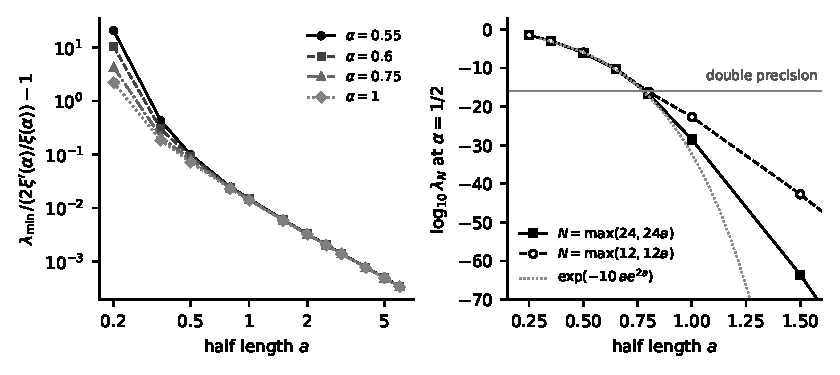
\includegraphics[width=0.95\textwidth]{fig/yo_lam.pdf}
\caption{Left: the excess of the least eigenvalue of the damped Yoshida form over its floor, $\lambda_{\min}(\alpha,a)/(2b_\alpha)-1$, against the window half length $a$, for $\alpha=0.55$, $0.6$, $0.75$, $1$ (finite sections of $\max(96,\lceil24a\rceil)$ modes, logarithmic scales); it tends to zero, roughly like $a^{-2}$. Right: $\log_{10}$ of the finite section value at $\alpha=\frac12$ for $N=\max(24,24a)$ and $N=\max(12,12a)$ modes, with the level of double precision and the curve $\exp(-10ae^{2a})$.}
\label{yo:fig:lam}
\end{figure}

Figure~\ref{yo:fig:symbol} shows the symbol on four lines.

\begin{figure}[htbp]
\centering
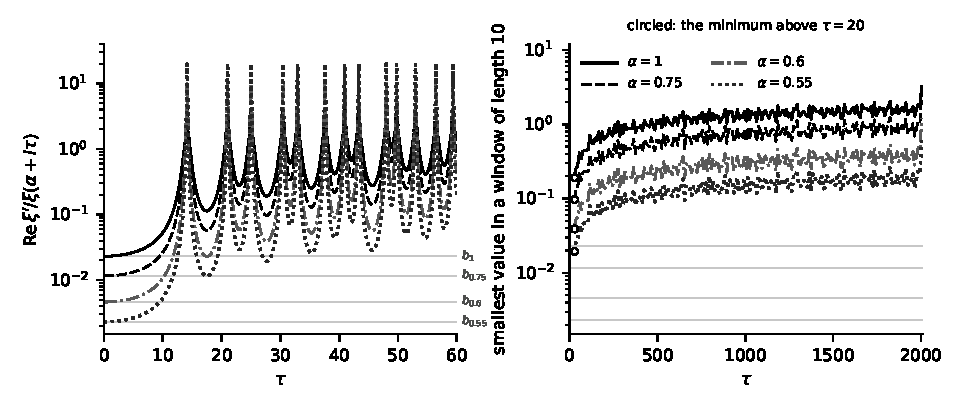
\includegraphics[width=0.95\textwidth]{fig/yo_symbol.pdf}
\caption{Left: the symbol $v_\alpha(\tau)=\re\xi'/\xi(\alpha+i\tau)$ on $[0,60]$ for $\alpha=1$, $0.75$, $0.6$, $0.55$ (logarithmic scale), with $b_\alpha$ as thin horizontal lines. Right: the smallest value of $v_\alpha$ in windows of length $10$ on $[0,2000]$, with the minimum above $\tau=20$ circled. Above $\tau=20$ the minima are $0.1901$, $0.0968$, $0.0389$ and $0.0195$ for $\alpha=1$, $0.75$, $0.6$, $0.55$, which are $8.2$, $8.4$, $8.4$ and $8.4$ times $b_\alpha$, all at $\tau=27.67$, between the third and the fourth ordinate (the largest gap above the second); the lowest local minimum other than the one at the origin is lower, $4.90\,b_1$ at $\tau=17.49$ for $\alpha=1$ and $4.98\,b_{0.55}$ for $\alpha=0.55$, in the gap between the first two ordinates.}
\label{yo:fig:symbol}
\end{figure}

At $\alpha=\frac12$ Theorem~\ref{yo:thm:coercive} does not apply. Under RH the symbol there is the atomic measure on the ordinates, the vague limit of $\rho_\varepsilon$ as $\varepsilon\downarrow0$; it vanishes between the atoms, which is why $\lambda_{\min}(\frac12,a)\to0$, and under RH the decay is faster than any power of $a$ (Theorem~\ref{dc:thm:ladder}(c) of Chapter~\ref{chap:dc}). The speed of the collapse in Table~\ref{yo:tab:lam} is a numerical observation. The finite section values at $\alpha=\frac12$ follow $\exp(-2c\,ae^{2a})$ with $c=-\log\lambda/(2ae^{2a})=4.12$, $4.77$, $5.10$, $5.01$, $4.86$ at $a=0.25$, $0.35$, $0.5$, $0.65$, $0.8$ (so $4.1\le c\le5.1$, at $N=48$). Zhu proves, under RH and for all large $a$, only the bound $\exp(-ae^a)$ for the least eigenvalue over real even test functions (Theorem 1.3 of \cite{Zhu26}, Chapter~\ref{chap:zhu}): it has $e^a$ where the observed decay has $e^{2a}$. For $a\ge1.5$ the finite sections saturate and $c$ falls, so those values say nothing about the infimum. A heuristic for the form of the decay: $\widehat\varphi$ is an entire function of exponential type $a$ and has at most about $2aH/\pi$ real zeros in $[-H,H]$, against about $(H/\pi)\log(H/2\pi)$ ordinates there, so a vector of type $a$ can vanish at every ordinate up to a height of about $2\pi e^{2a}$ and no further, which suggests a decay like $\exp(-c\,ae^{2a})$. This is not a proof.
